\documentclass[11pt]{article}
\usepackage{graphicx}
\usepackage{mathtools}
\usepackage{amssymb,amsmath}
\usepackage{textcomp}
\DeclareMathOperator*{\argmin}{arg\,min}

%\usepackage{subcaption}
%\usepackage{float}
\usepackage{setspace}
\usepackage{fullpage}
\usepackage[font=scriptsize]{caption}
%\usepackage{fullpage}
%\setcounter{secnumdepth}{1}
\begin{document}

\title{GRN inference in multiple species}
\author{Kari Y. Lam, Zachary M. Westrick, Others TBA}
\maketitle

\begin{abstract}
I'm MC Zack and I've got something to say. Hey. Hey. Hey. Hey. Hey
\end{abstract}

\section{Introduction}

\begin{figure}
\begin{center}
  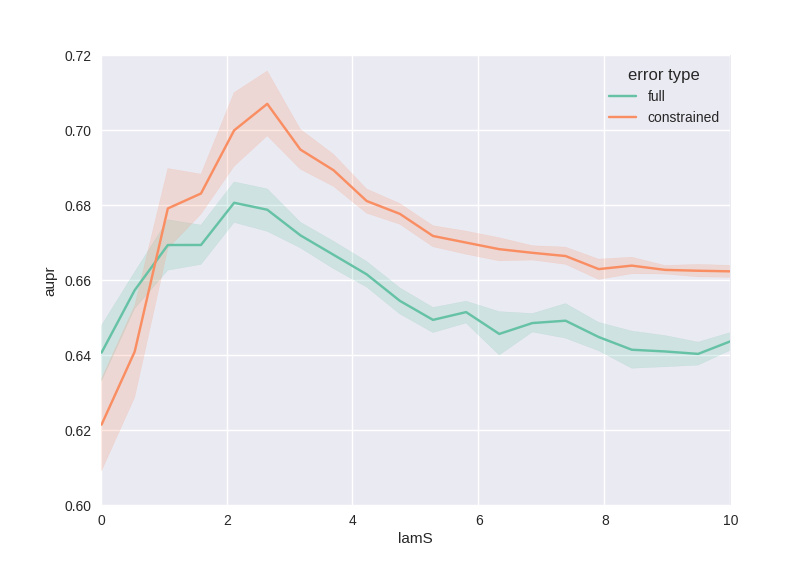
\includegraphics[scale=0.45]{simulated.png}
  \caption{\label{fig:figure1} This is what a figure looks like}
  \end{center}
\end{figure}

\section{Methods}
\subsection{GRN}
We model gene regulatory networks using ordinary differential equations where the change in expression of some gene $x_{i}$ is described as a linear combination of regulators:
\begin{equation}
\frac{\mathrm d}{\mathrm d t} = -\alpha_{i}x_{i} + \sum \beta_{i,j}x_{j}
\end{equation}
where $\alpha$ is the degradation rage and $\beta$ is a set of parameters to be estimated.

\noindent We approach the learning of the $\beta$ matrix using regression. We solve
\begin{equation}
\argmin_\beta\vert \vert X\beta - Y_2 \vert \vert ^2
\end{equation}
where the matrix $X \in R^{n \times k}$ is the expression matrix with $n$ conditions and $k$ transcription factors. $X$ is a submatrix of $Y \in R^{n \times m}$, the gene expression matrix with $m$ genes. Typically, $n < k < m$, so this problem is ill-posed without regularization. We use ridge regression and solve
\begin{equation}
\argmin_\beta\vert \vert X\beta - Y_2 \vert \vert ^2 + \lambda_R \vert \vert \beta \vert \vert ^2
\end{equation} 
with $\lambda_R$ as the weight of the regularization term.

\subsection{Fused GRN}
Related species are expected to be governed by similar but not necessarily identical gene regulatory networks. Pooling data from multiple species drowns out species-specific mechanisms, but learning GRNs separately limits the availability of training data. We approach the problem of cross-species GRN inference by learning networks simultaneously with an additional constraint in the form of an L2 penalty on differences between interactions between orthologous TF, gene pairs. The assumption is that orthologous genes play analogous roles in their respective GRNs, and therefore, the interactions between orthologous TF, gene pairs should have similar weights. \\

We solve
\begin{equation}
\argmin_\beta \vert \vert X^1 \beta^1 - Y_2 ^1 \vert \vert ^2 + \vert \vert X^2 \beta^2 - Y_2 ^2 \vert \vert ^2 + \lambda_R \vert \vert \beta^1 + \beta^2 \vert \vert ^2 + \lambda_S \sum\limits_{i^1, i^2, j^1, j^2 \in C} (\beta^1_{i^1,j^1} - \beta^2_{i^2,j^2})^2
\end{equation}
where $C$ is the set of orthologous TF, gene pairs.\newline

If $\lambda_S = 0$, this is equivalent to solving the two regression problems separately, while $\lambda_S = \infty$ corresponds to requiring equality between constrained entries of $B^1, B^2$ where in the case of 1 to 1 correspondence weights, this is equivalent to pooling the data for the two species and solving one regression problem. \\

We use an L2 norm because it can be solved in closed form and because the structure of differences between corresponding weights may not be sparse, but should simply be made small.

\subsection{Simulated data}
Generation of simulated data begins with the production of random orthology mappings. We produce a one-to-one orthology by pairing random genes until a specified fraction have been assigned orthologs. This process is carried out separately for TFs and non-TF genes, so that TFs and non-TF genes are never assigned to be orthologous. We then produce a pair of random networks ($B^1$ and $B^2$) as follows. For each unfilled entry in $B^1$ or $B^2$, we enumerate the set $C$ consisting of the entry along with every entry in either matrix to which it is fused. With probability equal to the sparsity rate we assign every entry in $C$ to be 0, otherwise we sample a value $v \sim \mathcal{N}(0,1)$ and independently assign each entry in $C$ to $v + \mathcal{N}(0, \sigma_f^2)$. $\sigma_f$ is a parameter that controls the distribution of differences in the values of fused coefficients, so that the nonzero coefficients of $B^1, B^2$ are distributed as $\mathcal{N}(0, 1 + \sigma_f^2)$.

Given a network $B$, we generate $N$ samples of gene expressions at each of two timepoints. The condition by gene expression matrix for timepoint one, $Y_{T1}$, is sampled randomly from a multivariate Gaussian distribution with identity covariance matrix. $X_{T1}$ is the TF expression sub-matrix of $Y_{T1}$, and consists of columns of $Y_{T1}$ that correspond to TFs. Treating the decay rate as 0, the gene expression matrix at timepoint two, $Y_{T2}$ is sampled as $Y_{T2} = Y_{T1} + BX_{T1}$. This process is carried out separately for each network. 

Following generation of simulated data, we may introduce error into the orthology mapping. This can take the form of discarding a specified fraction of true orthologies (governed by a false-negative rate), or by introducing random false orthologies (governed by a false-positive rate). For convenience, the false-positive rate is specified in units of the number of true orthologs, and not the number of possible orthologs. 

For the purposes of evaluating simulated network recovery, we define a gold standard network as the support of the beta matrices. Priors used in network inference are interactions from the gold standard. The list of priors can be be manipulated to include false positives and false negatives as with the generation of orthologs. 

\subsection{Bacterial data}
is good
Look an equation array
\begin{equation}
\begin{array}{l}
R_i^{\mathrm{input}}(\theta) = c g_i^{\mathrm{input}}\exp(-(\theta - \theta_i)^2 / (2\sigma^2_{\mathrm{input}}))
\\
R_i^{\mathrm{output}}(\theta) = g_i^{\mathrm{output}}\sum_{j=0}^N R_j^{\mathrm{input}}(\theta) \exp(-(\theta_i - \theta_j)^2/(2\sigma^2_{\mathrm{output}})) .
\end{array}
\end{equation}
\bibliographystyle{plain}
\bibliography{paper}

\end{document}

